\subsection{Speicherhierarchien 1}
Tabelle \ref{tbl:hirachy1} gibt die \textbf{Verzögerung} im Falle eines \textbf{erfolgreichen} Zugriffs auf die jeweilige Speicherebene an.

Der durchschnittliche CPI-Wert \underline{ohne} Berücksichtigung der Speicherzugriffe betrage 1,3 (idealer CPI). \textbf{20\%} aller Instruktionen greifen auf den Speicher zu.

\begin{table}[h!]
	\centering
	\begin{tabular}{lll}
		\hline
		Speicherebene & Hitrate & Verzögerung/Takte \\\hline
		L1 & 85\% & 4 \\
		L2 & 75\% & 12 \\
		RAM & 100\% & 236 \\\hline
	\end{tabular}
	\caption{Speicherebenen und Verzögerung in Takten}
	\label{tbl:hirachy1}
\end{table}

\begin{enumerate}[a)]
	\item \textbf{Durchschnittlicher CPI-Wert unter Berücksichtigung der Speicherzugriffe}
	\begin{figure}[h!]
		\centering
		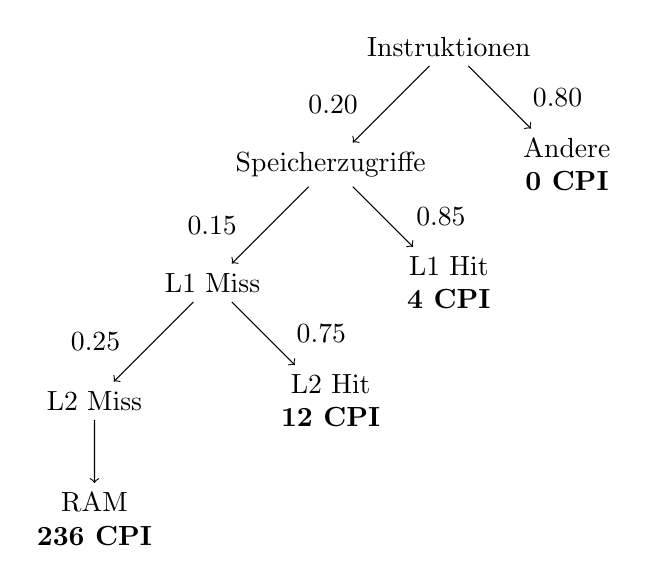
\begin{tikzpicture}
		\node{Instruktionen}[->]{
			child{node{Speicherzugriffe} 
				child{node{L1 Miss}
					child{node{L2 Miss}
						child{node[align=center]{RAM\\\textbf{236 CPI}}}
						edge from parent node[left=3mm]{0.25}
					}
					child[missing]
					child{node[align=center]{L2 Hit\\\textbf{12 CPI}}
						edge from parent node[right=3mm]{0.75}
					}
					edge from parent node[left=3mm]{0.15}
				}
				child[missing]
				child{node[align=center]{L1 Hit\\\textbf{4 CPI}}
					edge from parent node[right=3mm]{0.85}
				}
				edge from parent node[left=3mm]{0.20}
			}
			child[missing]
			child{node[align=center]{Andere\\\textbf{0 CPI}}
				edge from parent node[right=3mm]{0.80}
			}
		};
		\end{tikzpicture}
		\caption{Wahrscheinlichkeiten der Speicherzugriffe mit ihren \textbf{Verzögerungen}}
		\label{fig:prob1}
	\end{figure}

	Berechne die durchschnittliche Verzögerung aus Abbildung \ref{fig:prob1} durch gewichtete Aufsummierung der Knoten.
	\begin{equation}
		\overline{\text{Verzögerung}} = 0.8 \cdot 0 + 0.2 \cdot (0.85 \cdot 4 + 0.15 \cdot(0.75 \cdot 12 + 0.25 \cdot 236)) = 2.72
		\label{eq:avgdelay1}
	\end{equation}
	
	
	Addiere die durchschnittliche Verzögerung zum idealen CPI-Wert um den durchschnittlichen CPI-Wert unter Berücksichtigung der Speicherzugriffe zu erhalten.
	\begin{equation}
		\overline{\text{CPI}_\text{gesamt}} = \overline{\text{Verzögerung}} + 1.3 = 4.02
	\end{equation}
	
	
	\item \textbf{Prozent der Ausführungszeit, die der Prozessor auf Speicherzugriffe warten muss}
	
	Die durch Speicherzugriffe verursachte Verzögerung ist $ \overline{\text{Verzögerung}} = 2.72 $. Berechne das Verhältnis zum durchschnittlichen CPI-Wert.
	\begin{equation}
		\frac{\overline{\text{Verzögerung}}}{\overline{\text{CPI}_\text{gesamt}}} = \frac{2.72}{4.02} \approx 0.677
	\end{equation}
	
	
	\item \textbf{Hitrate des L1-Caches, um einen durchschnittlichen CPI-Wert von 3 zu erhalten}
	
	Die maximale Verzögerung, die nun durch Speicherzugriffe auftreten darf, ist $ \overline{\text{Verzögerung}} = 3 - 1.3 = 1.7 $.
	Man schreibe die Gleichung \ref{eq:avgdelay1} um und löse nach der Hitrate des L1 Caches $ p_\text{L1} $.
	\begin{align}
	\overline{\text{Verzögerung}} = 0.8 \cdot 0 + 0.2 \cdot (p_\text{L1} \cdot 4 + (1- p_\text{L1}) \cdot(0.75 \cdot 12 + 0.25 \cdot 236)) &= 1.7 \\
	 p_\text{L1} \cdot 4 + (1- p_\text{L1}) \cdot 68 &= \frac{1.7}{0.2} \\
	  4 \cdot p_\text{L1} - 68 \cdot p_\text{L1} &= 8.5 - 68 \\
	  p_\text{L1} &= \frac{-59.5}{-64} \\
	  &\approx 0.93
	\end{align}
\end{enumerate}